\section{Resisitive switch design}
\label{sec:resisitive_switch_design}
- Mechanical concept: Simple beam, contact pad, actuation pad
- Simplifications

\subsection{Basic concepts}
\label{sec:basic_concepts}
Area moment of inertia of recangular section:
\begin{equation}
	I_z = \frac{bh^3}{12}
	\label{eq:area_moment_of_inertia}
\end{equation}

Deflection of a beam:
\begin{figure}[h]
	\centering
	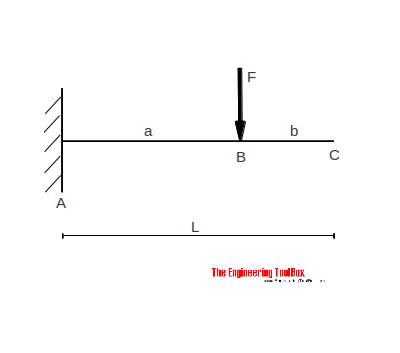
\includegraphics[width=8cm]{fig/cantilever_beam_single_load.png}
	\label{fig:cantilever_beam_single_load}
\end{figure}

\begin{equation}
	\delta = \frac{F}{3EI}\cdot\frac{a^3(1+3b)}{2a}
	\label{eq:beam_deflection}
\end{equation}

Effective mass:
\begin{equation}
	m_{eff} = \rho A \int_0^l{\left[\frac{y(x)}{y(l)_{max}}\right]^2dx}
	\label{eq:effective_mass}
\end{equation}


- Frequency response / Minimal switching
Spring constant:
\begin{equation}
	k = \frac{F}{\delta} = \frac{Ewt^3}{4L^3}
	\label{eq:spring_constant}
\end{equation}

Resonance frequency:
\begin{equation}
	\omega_0 = \sqrt{\frac{k}{m_{eff}}}
	\label{eq:resonance_frequency}
\end{equation}

Capacitance actuator pad:
\begin{equation}
	C = \frac{\varepsilon A}{d}
	\label{eq:plate_capacitor}
\end{equation}

- Electrostatic analysis / Force <-> Area
Note: Distance smaller than surface, neglect fringes because of aspect ratio
\begin{equation}
	F_{ES} = \frac{\varepsilon AV^2}{2d^2}
	\label{eq:electrostatic_force}
\end{equation}

- Electric properties of contacts
Resistance:
\begin{equation}
	R = \rho\frac{l}{wt}
	\label{eq:resistance}
\end{equation}

- Failure

- Thermal
Not critical blablabla 

\subsection{Analysis}
\label{sec:analysis}
- Actuation point vs contact point placement
- Area contact
- Area actuator
- Beam cross section
- Material
